\documentclass[11pt]{article}
\usepackage{amsmath}
\usepackage{graphicx}
\usepackage{multirow}
\usepackage{booktabs}
\usepackage{verbatim}
\usepackage{color}
\usepackage{hyperref}
\usepackage{url}
\usepackage{geometry}
\usepackage{esvect}
\usepackage{esdiff}
\usepackage{siunitx}
\usepackage{caption}
\usepackage{subfig}
\usepackage{textcomp, gensymb}
%\textwidth 17cm
%\evensidemargin -0.5cm
%\oddsidemargin -0.5cm
\geometry{margin=2.5cm}
%\setlength{\belowcaptionskip}{-10pt}

%TITLE PAGE WITH ABSTRACT AND ToC
\begin{document}
\title{Ganymede Surface Magnetic Field Analysis}
\author{Isaac Wetton}
\date{\today}
\maketitle

\section{Introduction}
\label{sec:intro}

This document details how I went about analysing the surface magnetic field strength of Ganymede using observed magnetic field data from the Galileo spacecraft. Section \ref{sec:meth} will describe the method employed to obtain magnetic field data plots and a result for the magnetic field at the surface of Ganymede so that the results may be reproduced, whilst section \ref{sec:result} will analyse the obtained data to draw conclusions on the surface magnetic field strength, discuss uncertainty in the result and any additional factors.

\section{Methodology}
\label{sec:meth}

Galileo spacecraft data was chosen as Galileo was a Jupiter orbiter which recorded measurements of magnetic field strengths and made multiple flybys of Ganymede \cite{craft}. The magnetic field data recorded by Galileo, alongside data for its position with respect to Jupiter and Ganymede, were retrieved from the \emph{Amda} website \cite{amda}. To determine the surface magnetic field strength of Ganymede, we opted to use observed data from Galileo's flyby of the satellite on 27\textsuperscript{th} December 2000 \cite{nasaflybys} as it had more frequent and more consistent measurements in comparison to previous flybys, and flew near to Ganymede's southern pole.

The measurements taken of magnetic field during the flyby have contributions from both Jupiter and Ganymede. To isolate Ganymede's magnetic field from Jupiter's contribution, multiple Python scripts, available in appendix \ref{app:scripts}, were written to first identify time frames in which Galileo was in approximately the same position as it was during the December 2000 flyby, then to modify one of these occasions' data to produce artificial Jupiter field data which could be subtracted to isolate Ganymede's field during the flyby.

\subsection{Identifying occasions with a similar Galileo position to December 2000's flyby}
The first Python script used an input text file containing position data from \emph{Amda} for Galileo's orbit of Jupiter from 1\textsuperscript{st} September 1996 to 1\textsuperscript{st} September 2003. If the position of the spacecraft was within approximately 5 Jupiter radii in each JSO direction of its position during the December 2000 flyby of Ganymede, then that data point was added to an output file. The position of Galileo during the December 2000 flyby was taken as its average across the stated time frame \cite{nasaflybys}, measured to be (-15.2, 0.57, 0.84) in JSO coordinates \cite{amda}.

The script identified a total of 7 additional occasions where Galileo was within the specified position range: 9\textsuperscript{th} October 1999, 24\textsuperscript{th} November 1999, 2\textsuperscript{nd} January 2000, 21\textsuperscript{st} February 2000, 20\textsuperscript{th} May 2000, 22\textsuperscript{nd} May 2001 and 5\textsuperscript{th} August 2001, each having a duration of between 6.5 and 17.5 hours. Timeseries of observed magnetic field strength at Galileo for the first six of these occasions are shown in figure \ref{fig:6panelmag}.

\begin{figure}[!htb]
    \centering
    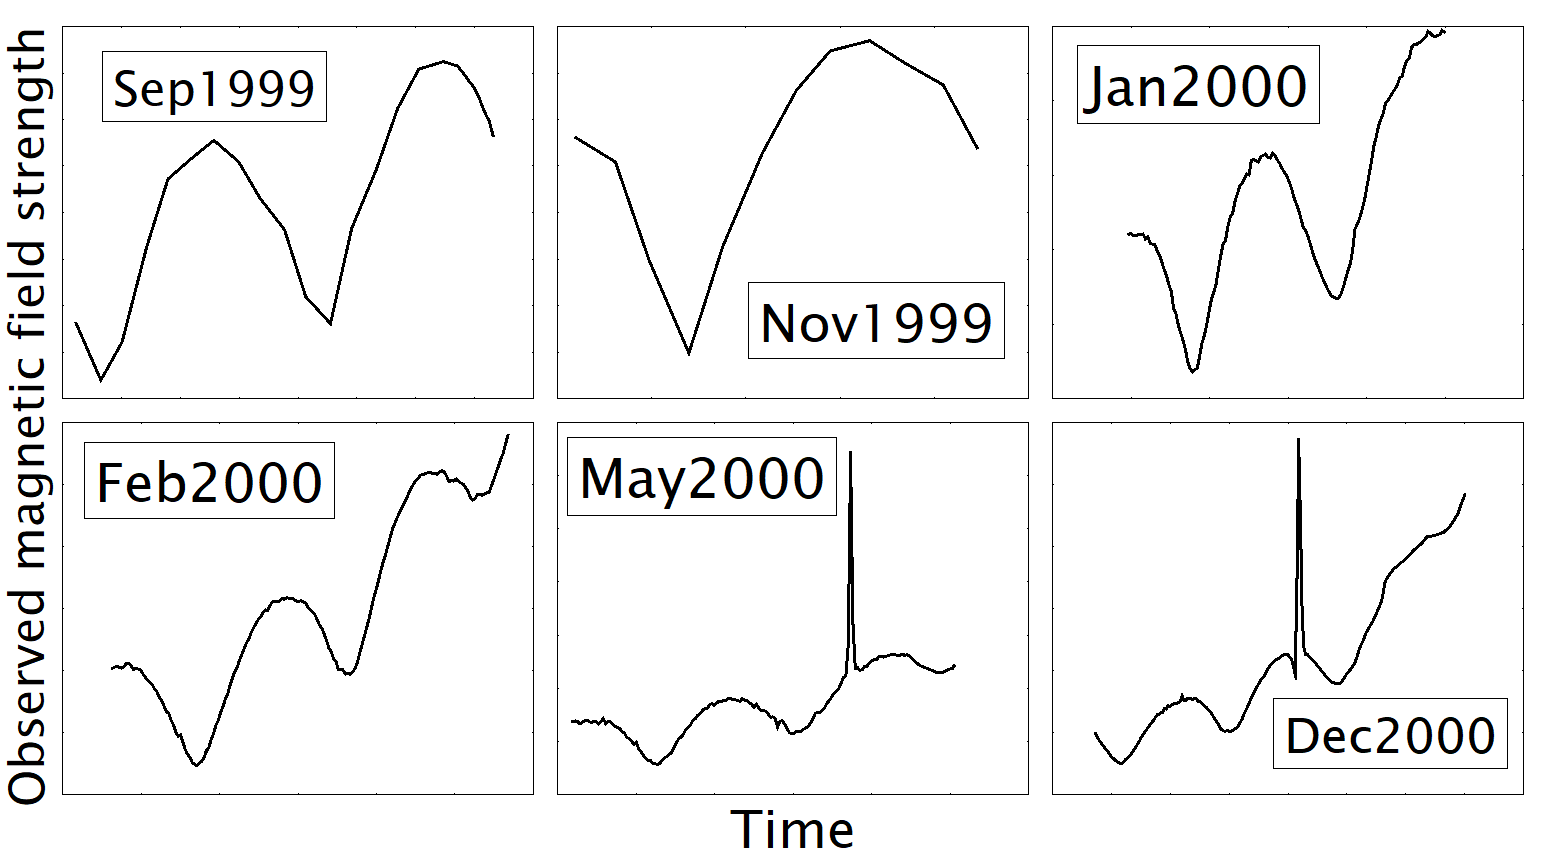
\includegraphics[width=8cm]{6magtimeseries-small.png}
    \captionsetup{width=13cm}
    \caption{Six timeseries of observed magnetic field magnitude by Galileo during six occasions where Galileo's position was similar to that of its December 2000 flyby of Ganymede. Moving across from top-left: 9\textsuperscript{th} October 1999, 24\textsuperscript{th} November 1999, 2\textsuperscript{nd} January 2000, 21\textsuperscript{st} February 2000, 20\textsuperscript{th} May 2000, 27\textsuperscript{th} December 2000.}
    \label{fig:6panelmag}
\end{figure}

\subsection{Isolating Ganymede's magnetic field from December 2000's flyby data}

Two new Python scripts were then written to remove Jupiter's contribution from the data. The May 2000 data was determined to have a non-flyby peak of similar magnitude to the December 2000 plot if the flyby spike was ignored, and so the script used May data to construct artificial December 2000 data for Jupiter's contribution only, which could then be subtracted from the December 2000 timeseries in figure \ref{fig:6panelmag} to effectively `isolate' Ganymede's field. The artificial data was created by calculating the difference between the May and December peaks when there was not a flyby, and adjusting the May data by the average distance. The script outputted an ASCII data file with values for time, magnetic field contribution and Galileo-Ganymede distance for the isolated Ganymede data.

Two plots were then produced - a timeseries of Ganymede's magnetic field contribution and a plot of Ganymede's magnetic field contribution against Galileo-Ganymede distance - for analysis of the field. The distance plot was solely for the Ganymede encounter period where there was a noticeable contribution from Ganymede, and included both the approach and retreat, with a fit of the form $\frac{A}{x^{3}} + B$ applied where $x$ is Galileo-Ganymede distance and $A$ and $B$ are constants. This particular fit was chosen as magnetic field strength from a dipole has an inverse cube law relationship with distance \cite{inversecube}, whilst also allowing for a potential base field due to other sources. The fit allowed for extrapolation to estimate the surface field at a distance of 1 Ganymede radius using the determined values of $A$ and $B$.

\subsection{Consideration of Ganymede's magnetic field rotation when comparing to expected results}

During the December 2000 flyby of Ganymede, Galileo flies close to the geographic north pole of Ganymede \cite{flybylines}. However, the magnetic north pole is rotated by $176 \pm 1\degree$ with respect to Jupiter's spin axis and $24 \pm 1\degree$ from the Jupiter-facing meridian plane toward the trailing hemisphere \cite{magrotation}. This must be accounted for to adjust the expected value before it can be compared to the surface field estimate we have obtained.

\subsection{Analysis of the May 2000 flyby data and estimation of surface magnetic field strength at Ganymede}
It can be seen from figure \ref{fig:6panelmag} that the May 2000 data also includes a flyby of Ganymede, characterised by the large spike in observed magnetic field strength at Galileo. This flyby specifically occurred on 2000-05-20 \cite{nasaflybys}, and occurred in a similar position with respect to Jupiter (within 5 Jupiter radii in each JSO coordinate as discussed) as the December 2000 flyby. The May flyby, however, crossed near to the geographic equator \cite{flybylines}.

The method used for obtaining a surface magnetic field strength at Ganymede for the December flyby was used to also obtain a value for the May flyby. The February 2000 data from approximately the same position with respect to Jupiter was used to create the artificial May data as it was determined to have a non-flyby peak of similar magnitude to the Jupiter field in May. The rotation of Ganymede's magnetic field was then taken into account and it was compared to the expected value from literature.

\section{Results \& Analysis}
\label{sec:result}

%REFERENCES PAGE
\newpage
\bibliographystyle{unsrt}
\bibliography{bibliography.bib}

\newpage
\appendix
\section{Python Scripts}
\label{app:scripts}
Python script(s) for identifying occasions with a similar Galileo position to December 2000's flyby: \url{https://github.com/IMAGINE-Lancaster-University/IMAGINE/tree/main/Data\%20Python\%20Scripts/JSOpositiondata}.

\noindent Python script(s) for constructing artificial magnetic field data and removing Jupiter's magnetic field contribution: \url{https://github.com/IMAGINE-Lancaster-University/IMAGINE/tree/main/Data\%20Python\%20Scripts/GanymedeIsolation}.

\end{document}
